\newcommand{\TeamNo}{31}

\newcommand{\HWno}{03}

\newcommand{\AuthorOneName}{Merve Nur Öztürk}
\newcommand{\AuthorOneID}{2311322}

\newcommand{\AuthorTwoName}{Atakan Süslü}
\newcommand{\AuthorTwoID}{2311371}

\newcommand{\AuthorThreeName}{Betül Rana Kuran}
\newcommand{\AuthorThreeID}{2311173}


\documentclass[letterpaper,12pt]{article}
\usepackage{tabularx} % extra features for tabular environment
\usepackage{amsmath}  % improve math presentation
\usepackage{amssymb}
\usepackage{xcolor}
\usepackage{float}
\usepackage[export]{adjustbox}
\usepackage{graphicx} % takes care of graphic including machinery
\usepackage[margin=1in,letterpaper]{geometry} % decreases margins
\usepackage{cite} % takes care of citations

\begin{document}
\begin{center}
AE 305, 2020-21 Fall \hfill \textbf{HW \HWno} \hfill \textbf{Team \TeamNo} \\
\noindent\rule{\textwidth}{0.4pt}
\begin{tabular}{p{0.33\textwidth} | p{0.33\textwidth} | p{0.33\textwidth} }
	\AuthorOneName&\AuthorTwoName&\AuthorThreeName\\
	\textit{\AuthorOneID}&\textit{\AuthorTwoID}&\textit{\AuthorThreeID}
\end{tabular}
\noindent\rule{\textwidth}{0.4pt}
\end{center}

%Report start

\section{Introduction}
\label{section:intro}

Finite Volume Method is a numerical method used in order to solve partial differential
equations representing the conservation of a quantity. In this homework, a potential flow
field over a circular cylinder at various values of angle of attack and a symmetric NACA
airfoil at zero angle of attack is requested to be calculated. For a potential flow,
the velocity field is obtained by the Laplace's equation:

\begin{equation}
	\vec{\nabla} \cdot \vec{\nabla}\phi = \frac{\partial^2 \phi}{\partial x^2} + \frac{\partial^2 \phi}{\partial y^2} = 0.
\end{equation}

\begin{equation}
\vec{V} = \vec{\nabla}\phi
\end{equation}

A pseudo time derivative is introduced in order to solve this equation without a system
of linear algebraic equations.

\begin{equation}
	\frac{\partial \phi}{\partial t} = \nu \left(\frac{\partial^2 \phi}{\partial x^2} + \frac{\partial^2 \phi}{\partial y^2}\right)
\end{equation}

where $\nu$ is an artificial diffusion coefficient. Steady-state boundary conditions are
set to calculate the steady-state solution as the time derivative goes to zero during the
integration. The integral form of the above equation is:

\begin{equation}
	\frac{\partial}{\partial t} \int_{\Omega}\phi  d\Omega + \oint_{S} \vec{F} \cdot d\vec{S} = 0
\end{equation}

\begin{equation}
	\vec{F} = -\nu\frac{\partial \phi}{\partial x}\vec{i} - \nu\frac{\partial \phi}{\partial y}\vec{j}
\end{equation}

Two boundary conditions are set such that the velocity is equal to the free stream velocity
far away from the body (Farfield BC) and there is no flow normal to the body, which is no
penetration boundary condition (Wall BC):

\begin{eqnarray}
	\vec{\nabla}\phi|_{far BC} &=& \vec{V}_{\infty} = \vec{u}_{\infty}\vec{i} + \vec{v}_{\infty}\vec{j} = V_{\infty}(cos\alpha\vec{i}+sin\alpha\vec{j})\\
	&=& V_{\infty}cos\alpha\vec{i} + V_{\infty}sin\alpha\vec{j}
\end{eqnarray}

\begin{equation}
	(\vec{n}\cdot\vec{V}_{\infty})_{wall} = 0 \:\mbox{or}\: (\vec{F}\cdot\vec{S})_{wall} = 0.
\end{equation}

The conserved quantity for this problem is the potential $\phi$, and the FV method is applied
for the calculation of this quantity as explained above.\\
\newpage
In this homework, Bernoulli's Equation is also used to calculate the pressure coefficient. Bernoulli's equation
implies that for inviscid, irrotational, and incompressible flows, when body forces are neglected,
the total pressure is constant at every point in the flow. The total pressure is equal to the summation of 
static and dynamic pressures.
\begin{eqnarray}
	P_1+q_1&=&P_2+q_2 \nonumber \\
	P_1+\frac{1}{2}\rho_1V_{1}^{2}&=&P_2+\frac{1}{2}\rho_2V_{2}^{2}\:=\:\mbox{constant}
	\label{eqn:bernoulli}
\end{eqnarray}
The pressure coefficient is calculated by
\begin{equation}
C_p=\frac{P-P_\infty}{q_\infty}
	\label{eqn:C_p}
\end{equation}
By substituting Equation \ref{eqn:bernoulli} and Equation \ref{eqn:C_p}, $C_p$ equation becomes
\begin{eqnarray}
	C_p&=&\frac{q_\infty-q}{q_{\infty}} \nonumber \\
	&=&1-\frac{q}{q_{\infty}}   \nonumber \\
	C_p&=&1-\frac{V^2}{V_{\infty}^{2}} 
	\label{eqn:C_p_new}
\end{eqnarray}


\section{Method}
\subsection{Finite Volume Method} 
In this homework, Finite Volume Method is used. In this method, an integral conservation law
\begin{equation}
        \frac{\partial}{\partial t}\int_{\Omega_e} q\,d\Omega + \oint_{S_e} \vec{F} \cdot \vec{dS} =0     
        \label{eqn:fvm}
\end{equation}
is applied to each control volume $\Omega_e$, and its boundaries $S_e$ in a discrete form. First, the solution domain is divided into small triangular cells and a computational mesh is created. 
Then, all cells are labeled and neighbour cells to their surfaces are identified. Then, conservation law is applied to all cells.\\
A pseudo time derivative is substituted into Laplace's equation which is multiplied by artificial
diffusion coefficient,$\nu$. The equation becomes
\begin{equation}
        \frac{\partial \phi}{\partial t} - \nu \vec{\nabla}\cdot\vec{\nabla}\phi = 0
        \label{eqn:pseudodiff}
\end{equation}
where $\vec{F}=-\nu\vec{\nabla}\phi$\\
Since a steady-state solution is obtained as the derivative goes to zero and steady boundary conditions 
are specified, Laplace’s equation is satisfied. 
The integral form of Equation \ref{eqn:pseudodiff} becomes
\begin{eqnarray}
        \frac{\partial}{\partial t}\int_{\Omega} \phi\,d\Omega + \oint_S \vec{F} \cdot \vec{dS} =0\ \\
        \mbox{where}\: \vec{F}=f\vec{i}+g\vec{j}=-(\nu\frac{\partial \phi}{x}\vec{i}+\nu\frac{\partial \phi}{y}\vec{j})\nonumber
        \label{eqnarray:genel}
\end{eqnarray}
Equation \ref{eqn:fvm} and Equation 14 have the same form. Therefore, the finite volume method can be applied.\\
A simple discrete form of Equation 14 applied to a two-dimensional triangular cell $e$ is then given by
\begin{equation}
        \frac{d(\phi_e\Omega_e)}{t}+\sum_{s=1}^{3} (\vec{F} \cdot \vec{dS})\ =0
        \label{eqn:diff}
\end{equation}
where $\phi_e$ is the average $\phi$ over element e, $\Omega_e$ is the area of triangle $e$ ,and
$\vec{S} = \Delta y_{e,s}\vec{i}-\Delta x_{e,s}\vec{j}$\\
In this homework, the averaging of cell-based quantities approach is used to calculate flux values. According to this approach,
the averages of the cell-based flux values of the cells sharing the same surface should be taken to compute the flux
through this surface. Therefore, the second term of \ref{eqn:diff} becomes
\begin{eqnarray}
	\sum_{s=1}^{3} (\vec{F} \cdot \vec{dS})&=&\sum_{s=1}^{3} (\vec{F_{e,s}} \cdot \vec{dS_{e,s}}) \nonumber \\
	&=&\sum_{s=1}^{3}[\frac{1}{2}(f_{e}+f_{e,ns})\Delta y_{e,s}-\frac{1}{2}(g_{e}+g_{e,ns})\Delta x_{e,s}] 
\end{eqnarray}

Equation \ref{eqn:diff} for element e becomes
\begin{equation}
        \Omega_e \frac{d\phi_e}{dt} +\sum_{s=1}^{3} [f_{e,s}\Delta y_{e,s}-g_{e,s}\Delta x_{e,s}]=0
\end{equation}
By using Taylor Series Expansion in time, the time derivative is approximated. These steps lead to the explicit Euler time
integration:
\begin{equation}
        \phi_{e}^{k+1} =\phi_{e}^{k} - \frac{\Delta t}{\Omega_e}\sum_{s=1}^{3}[f_{e,s}^{k}\Delta y_{e,s}-g_{e,s}^{k}\Delta x_{e,s}]
\end{equation}
Since $\vec{F}$ is diffusive flux, the average gradient vectors are calculated by
\begin{eqnarray}
\bar{\frac{\partial \phi}{\partial x}}\bigg|_{e}&=&\frac{1}{\Omega_e}\sum_{s=1}^{3}\frac{1}{2}(\phi_e+\phi{ns})\Delta y_{e,s} \nonumber \\
\bar{\frac{\partial \phi}{\partial y}}\bigg|_{e}&=&-\frac{1}{\Omega_e}\sum_{s=1}^{3}\frac{1}{2}(\phi_e+\phi{ns})\Delta x_{e,s}	\nonumber
\end{eqnarray}
\newpage

\section{Results and Discussion}

\subsection{Flowfield Around A Cylinder}

\begin{figure} [ht]
	\centering
	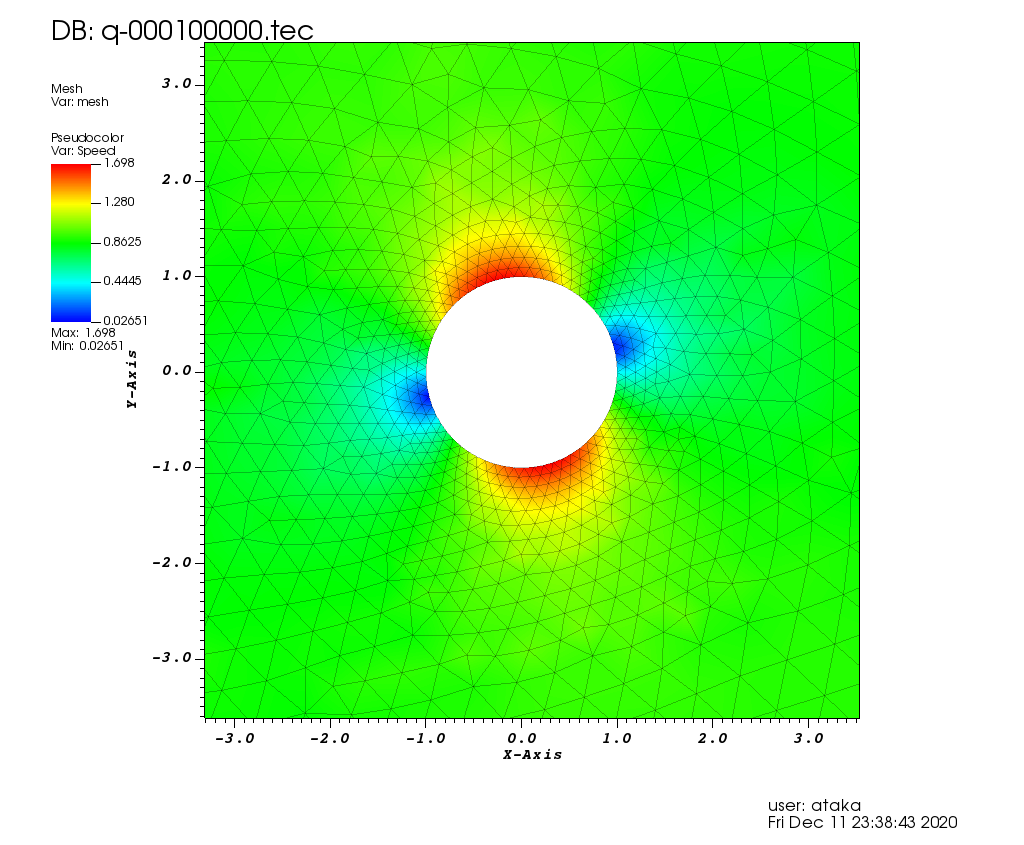
\includegraphics[height = 10cm]{graph/15deg/Cylinder_15angle_speed0001.png}
	\caption{Potential flow over a circular cylinder at $\alpha=15$ calculated by FV method.}
    \label{fig:q1p}
\end{figure}

\vspace{1cm}

According to the boundary conditions mentioned in Section \ref{section:intro}, FV fortran code
is completed. Afterwards, the flowfield around a cylinder is calculated using the unstructured grid provided.

\newpage

\subsection{Flowfield Around A Cylinder with Different Angle of Attacks}
\begin{figure} [ht]
	\centering
	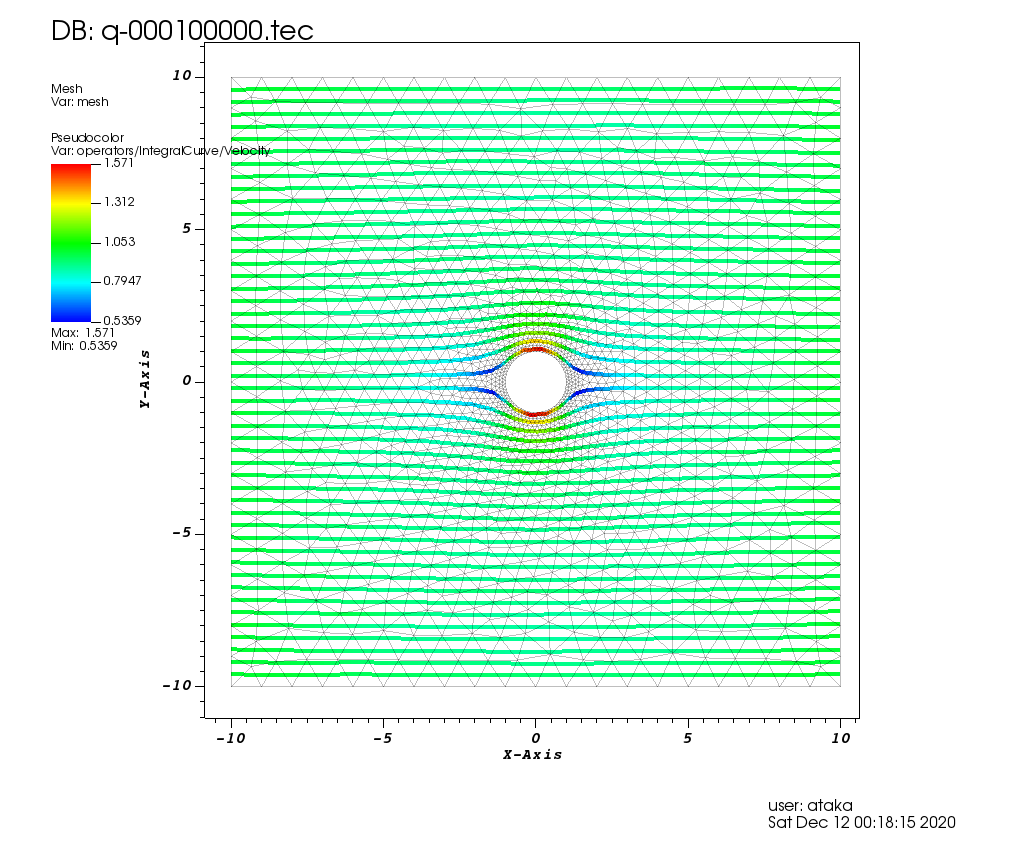
\includegraphics[height = 9.5cm]{graph/0deg/Cylinder_0angle_streamline0000.png}
	\caption{Streamlines over a circular cylinder at $\alpha=0$ calculated by FV method.}
    \label{fig:q2st0}
\end{figure}

\vspace{1cm}

In Figure \ref{fig:q2st0},\ref{fig:q2st15}, and \ref{fig:q2st-15}, it can be observed that streamlines
are parallel and horizontal lines far from the cylinder, and they are in the direction of the free stream velocity,
which results from the Farfield boundary condition. However, as approached the cylinder, streamlines are squeezed.
Moreover, they do not cross on each other and through the cylinder, since the normal component of velocity at
the surface of the cylinder is equal to zero. This is a consequence of the no penetration boundary condition, which
is also called the Wall boundary condition.

\newpage

\begin{figure} [!h]
	\centering
	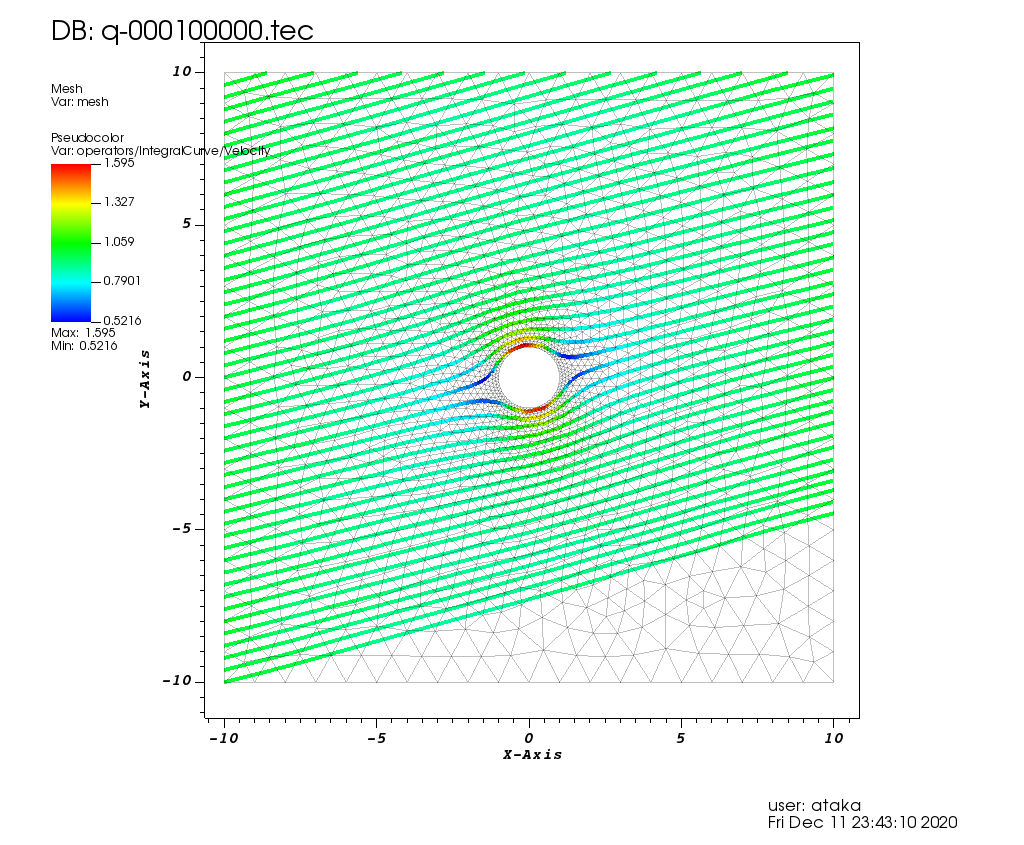
\includegraphics[height = 9.5cm]{graph/15deg/Cylinder_15angle_streamline0000.png}
	\caption{Streamlines over a circular cylinder at $\alpha=15$ calculated by FV method.}
    \label{fig:q2st15}
\end{figure}

\begin{figure} [!h]
	\centering
	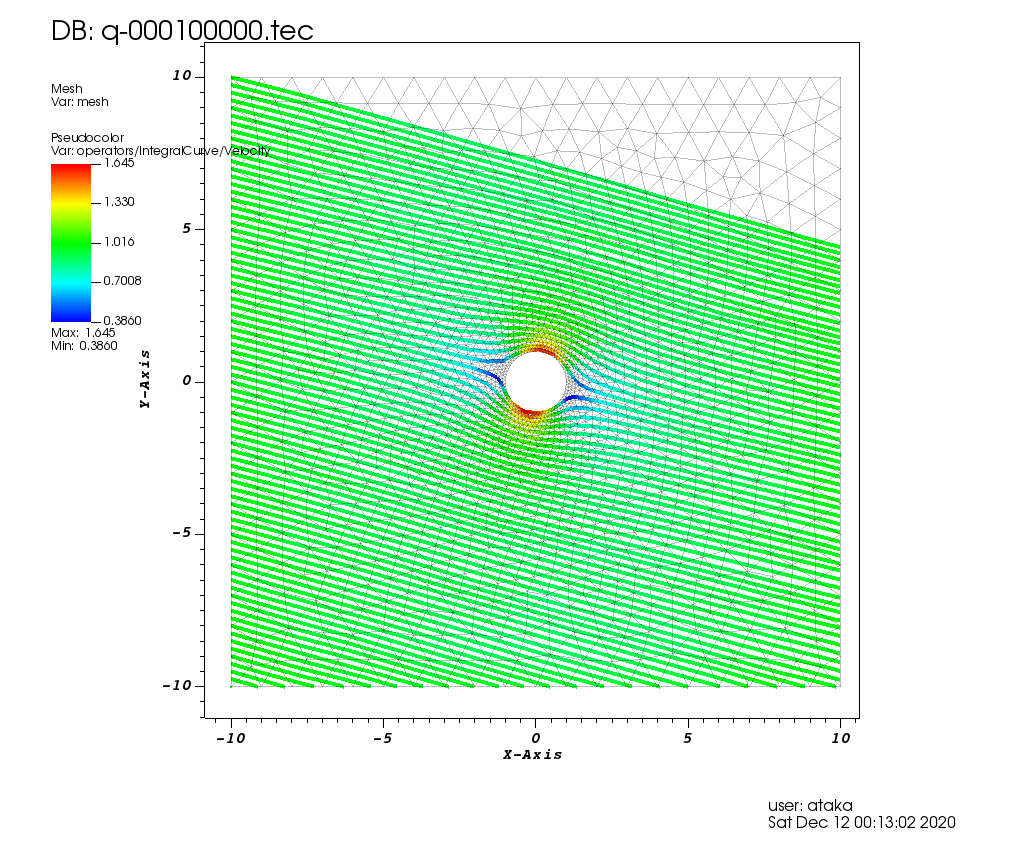
\includegraphics[height = 9.5cm]{graph/neg15deg/Cylinder_neg15angle_streamline0000.png}
	\caption{Streamlines over a circular cylinder at $\alpha=-15$ calculated by FV method.}
    \label{fig:q2st-15}
\end{figure}

\newpage

\begin{figure} [!h]
	\centering
	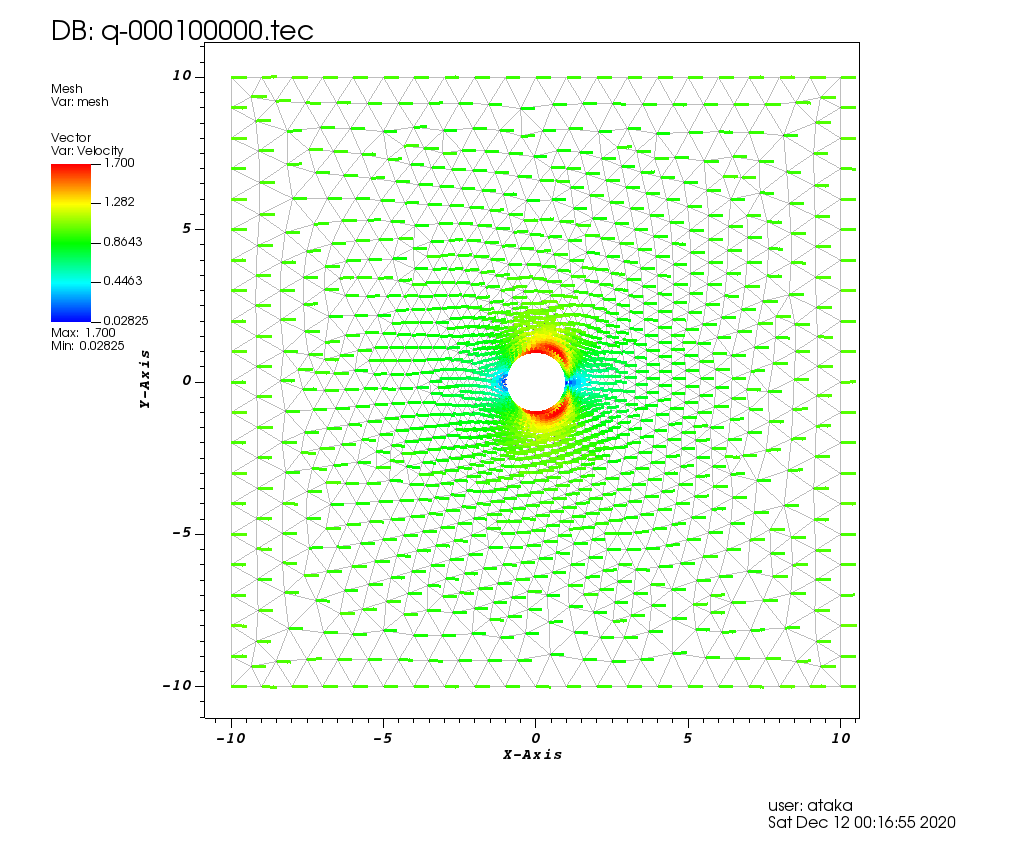
\includegraphics[height = 9.5cm]{graph/0deg/Cylinder_0angle_vector0000.png}
	\caption{The velocity vectors over a circular cylinder at $\alpha=0$ calculated by FV method.}
    \label{fig:q2v0}
\end{figure}

\begin{figure} [!h]
	\centering
	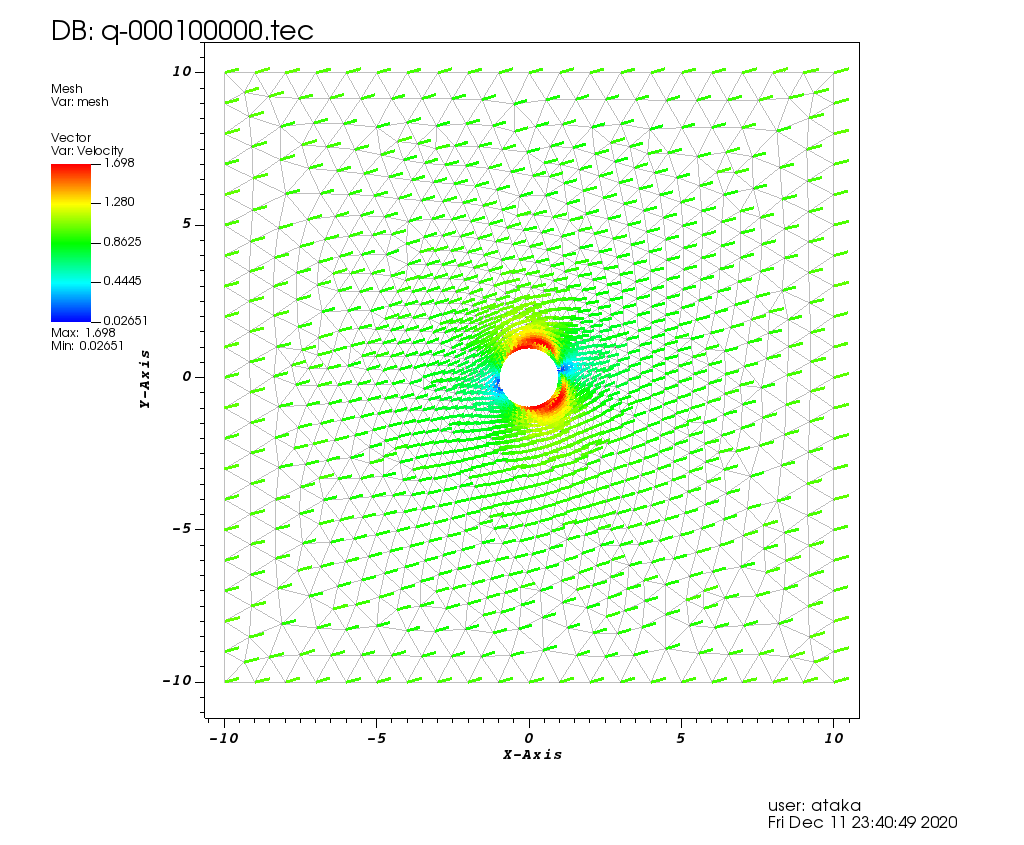
\includegraphics[height = 9.5cm]{graph/15deg/Cylinder_15angle_vector0000.png}
	\caption{The velocity vectors over a circular cylinder at $\alpha=15$ calculated by FV method.}
    \label{fig:q2v15}
\end{figure}

\newpage

\begin{figure} [ht]
	\centering
	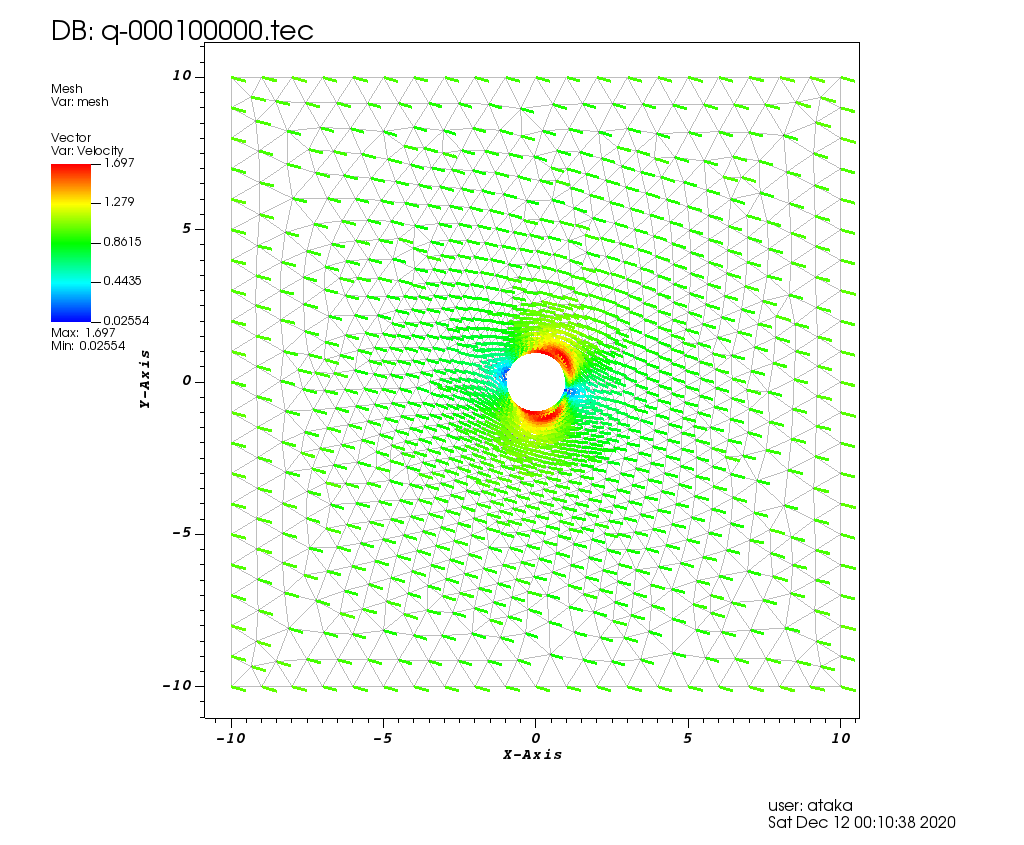
\includegraphics[height = 9.5cm]{graph/neg15deg/Cylinder_neg15angle_vector0000.png}
	\caption{The velocity vectors over a circular cylinder at $\alpha=-15$ calculated by FV method.}
    \label{fig:q2v-15}
\end{figure}

\vspace{1cm}

According to Figure \ref{fig:q2v0},\ref{fig:q2v15},and \ref{fig:q2v-15}, velocity vectors 
have the same direction, and magnitudes ($\vec{V}_{\infty}$) far from cylinder, which 
satisfies the Farfield boundary condition. Also, the velocity vectors near the cylinder are tangent
to the boundary. On the front and back of the cylinder, there are two points where the direction
of the velocity vector is too close to the normal of the surface. However, the magnitude of velocity is
so small that it can be considered as zero, satisfying the Wall boundary condition. These points
are called stagnation points.

\newpage

\subsection{Pressure Coefficient Distribution Over the Cylinder}
\begin{figure} [ht]
	\centering
	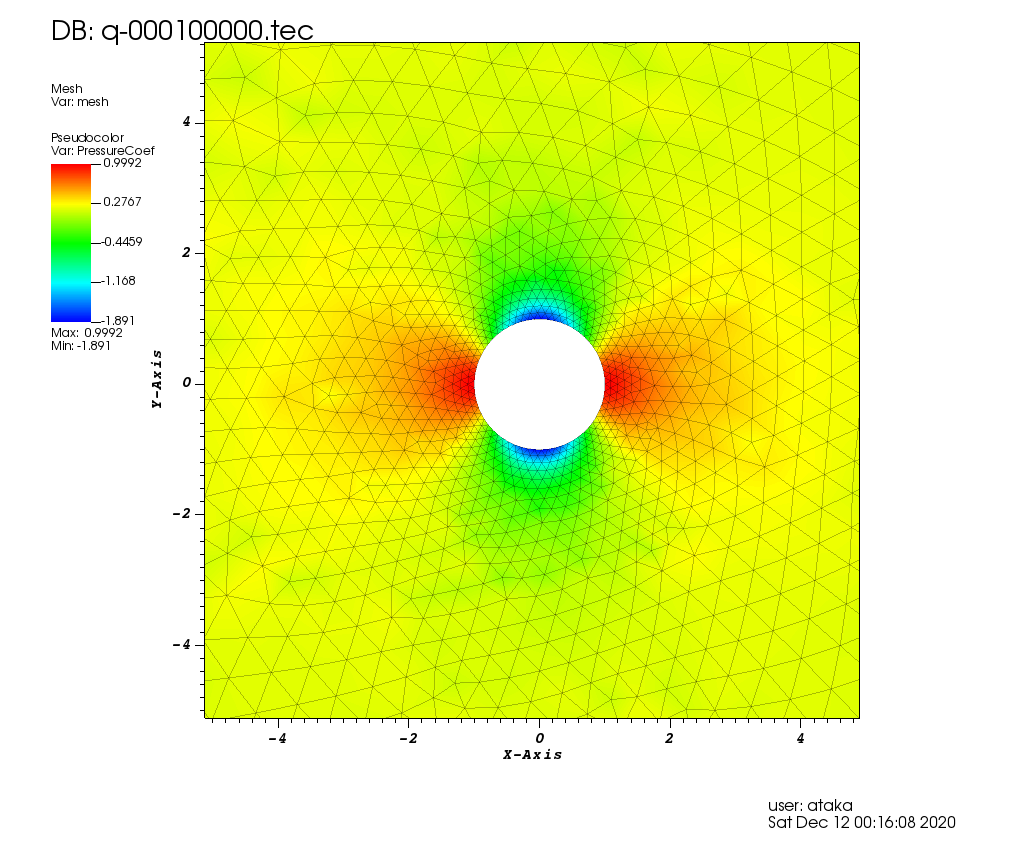
\includegraphics[height = 9.5cm]{graph/0deg/Cylinder_0angle_pressure0001.png}
	\caption{The pressure coefficient distribution over the circular cylinder at $\alpha=0$ calculated by FV method.}
	\label{fig:q3fv}
\end{figure}
\begin{figure} [ht]
	\centering
	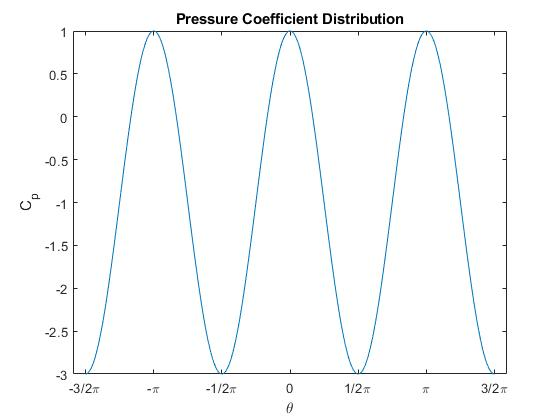
\includegraphics[height = 9.5cm]{graph/0deg/pc_analytical.jpg}
	\caption{The analytical solution of the pressure coefficient distribution over the circular cylinder at $\alpha=0$.}
	\label{fig:q3a}
\end{figure}

\newpage
In Figure \ref{fig:q3fv}, the pressure coefficient over the cylinder is calculated by using the 
Bernoulli's Equation and the FV method. On the other hand, in Figure \ref{fig:q3a}, the pressure coefficient
over the cylinder is plotted by the analytical solution. As can be seen from Figure \ref{fig:q3fv} 
The highest pressure coefficient is calculated at the front half and rear half of the cylinder, whereas
the lowest pressure coefficient is computed at the upper half and lower half of the cylinder. This result
coincides with the analytical solution. Since stagnation points, where velocities are equal to zero, 
are at the front and rear halves of the cylinder, from Equation 11, the highest pressure
coefficients are observed at these halves.

\subsection{NACA0012 airfoil mesh}
\label{sec:medium}

\begin{figure} [!h]
	\centering
	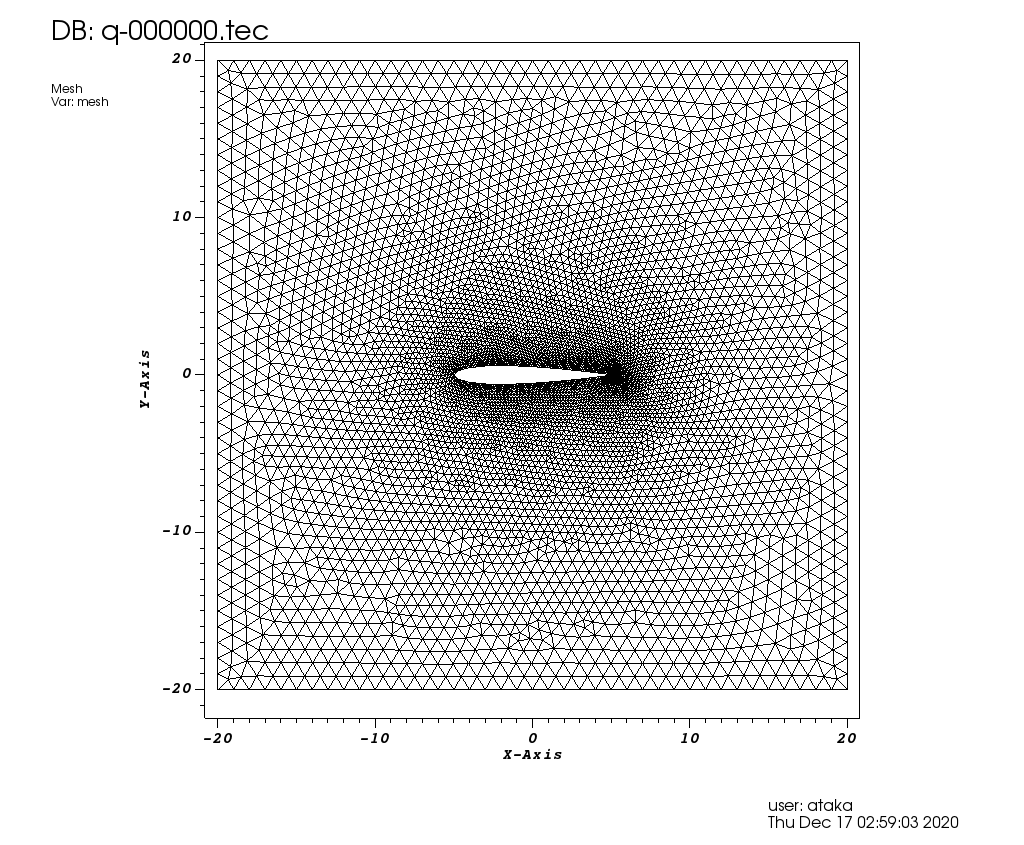
\includegraphics[height = 9.5cm]{graph/medium/medium_62650000.png}
	\caption{Unstructured mesh of NACA0012 airfoil}
    \label{fig:airfoilmesh}
\end{figure}

\vspace{1cm}

Unstructured mesh of NACA0012 airfoil is generated using Easymesh software. This
unstructured mesh consists of 6265 triangular grids.

\newpage

\begin{figure} [!h]
	\centering
	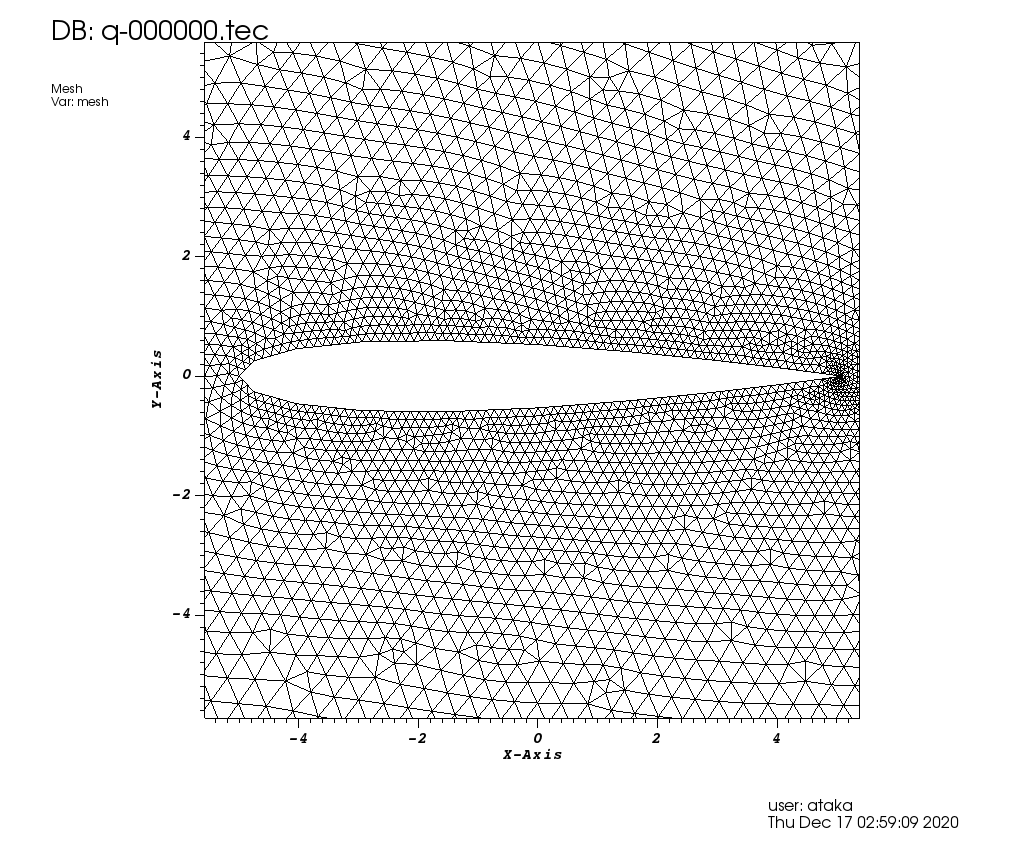
\includegraphics[height = 9.5cm]{graph/medium/medium_62650001.png}
	\caption{Unstructured mesh of NACA0012 airfoil near the airfoil}
    \label{fig:airfoilmeshclose}
\end{figure}

\vspace{1cm}

It can be seen from Figure \ref{fig:airfoilmesh} and Figure \ref{fig:airfoilmeshclose} that, the grids around
the airfoil are smaller for better accuracy, whereas the grids far from the airfoil are relatively bigger.
\newpage

\subsection{Pressure distribution around NACA0012 airfoil at $\alpha = 0$}

\begin{figure} [!h]
	\centering
	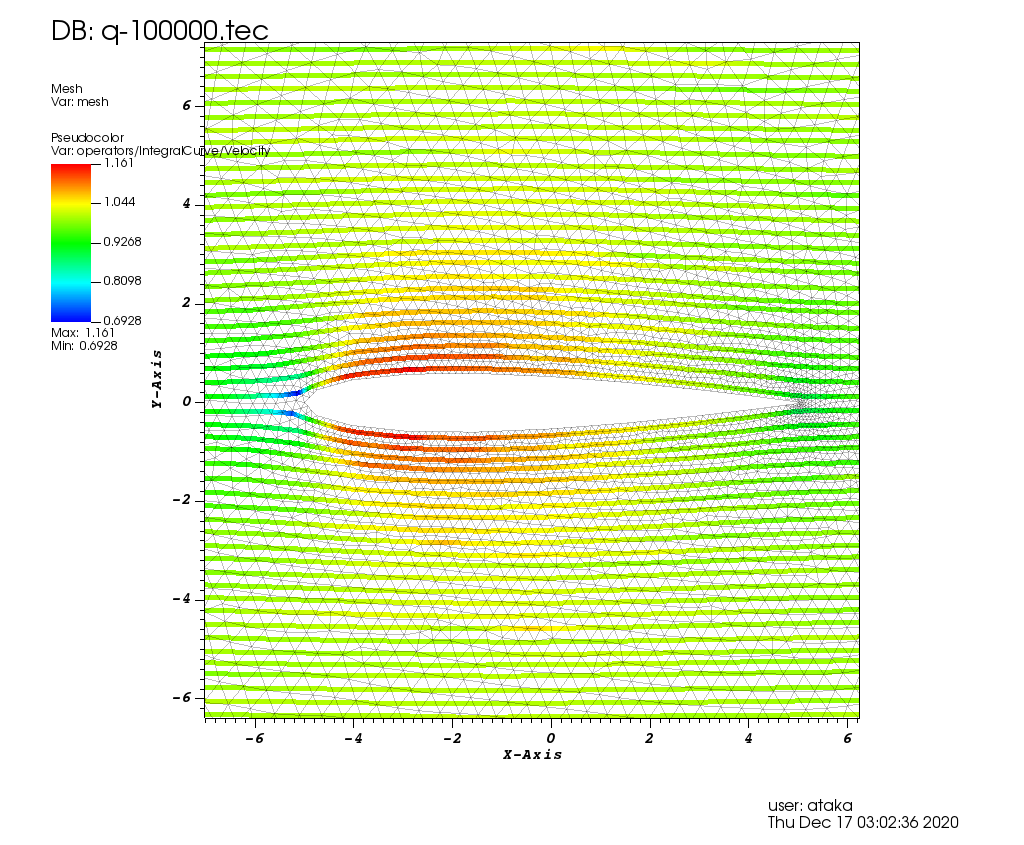
\includegraphics[height = 9.5cm]{graph/medium/medium_streamline0000.png}
	\caption{Streamlines around NACA0012 airfoil}
    \label{fig:airfoilstreamline}
\end{figure}

\vspace{1cm}

When the potential flow equation is solved using the Finite Volume Method and unstructured mesh in Figure \ref{fig:airfoilmesh},
flow around NACA0012 airfoil can be found. This flow can be illustrated using streamlines, as can be seen in 
Figure \ref{fig:airfoilstreamline}. As expected, air flows faster around the thicker sections of the airfoil, 
and air stagnates at the leading edge and the trailing edge. Moreover, the pressure coefficient can be calculated using Bernoulli's Equation
as the speed of the flow is known.

\newpage

\begin{figure} [!h]
	\centering
	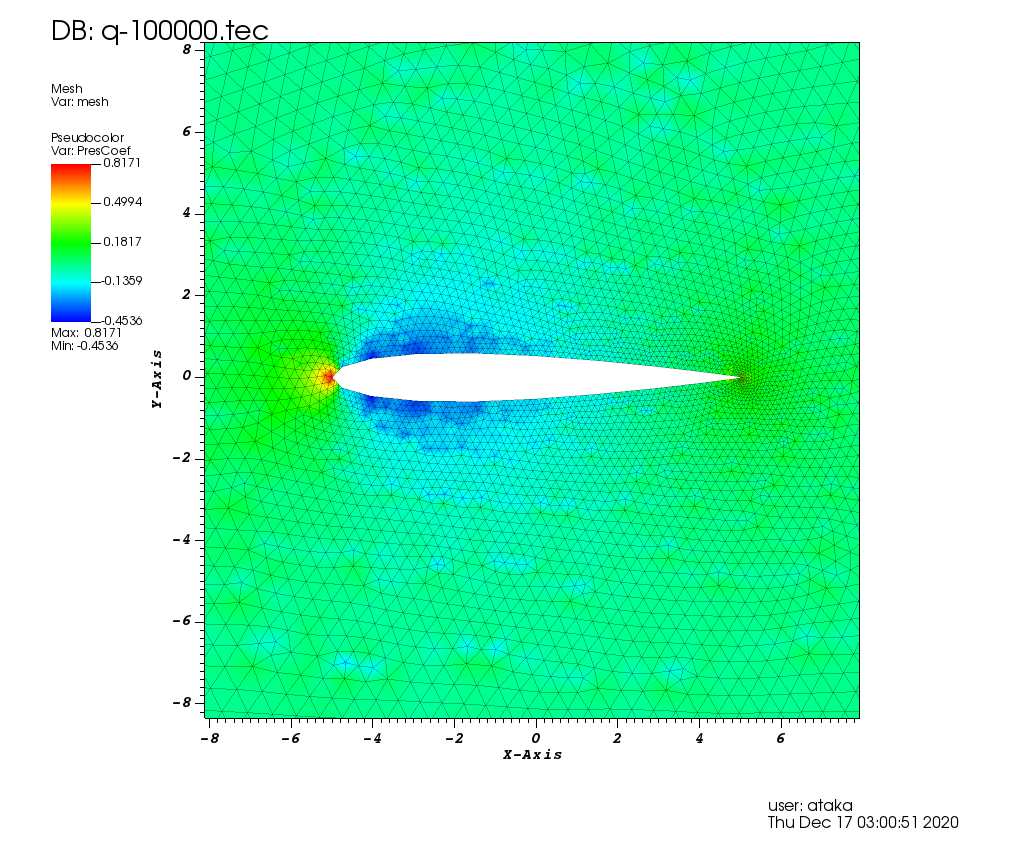
\includegraphics[height = 9.5cm]{graph/medium/medium_pressure0000.png}
	\caption{Pressure coefficient around NACA0012 airfoil}
    \label{fig:airfoilpressure}
\end{figure}

\vspace{1cm}

It can be seen from Figure \ref{fig:airfoilpressure} that pressure distribution on the upper and the lower surfaces are the same.
This is because airfoil is symmetric and airfoil is at zero angle of attack. If the angle of attack was different from zero, 
pressure distribution on the upper and lower surfaces would be different. It can also be seen that at the leading edge and the trailing edge,
the pressure is relatively larger; and around the maximum thickness, the pressure is relatively lower. This is because air flows slower at the
leading and the trailing edge and flows faster at the thicker part of the airfoil.
\newpage

\subsection{Solutions with different grid sizes}

\subsubsection{Coarse grid}

\begin{figure} [!h]
	\centering
	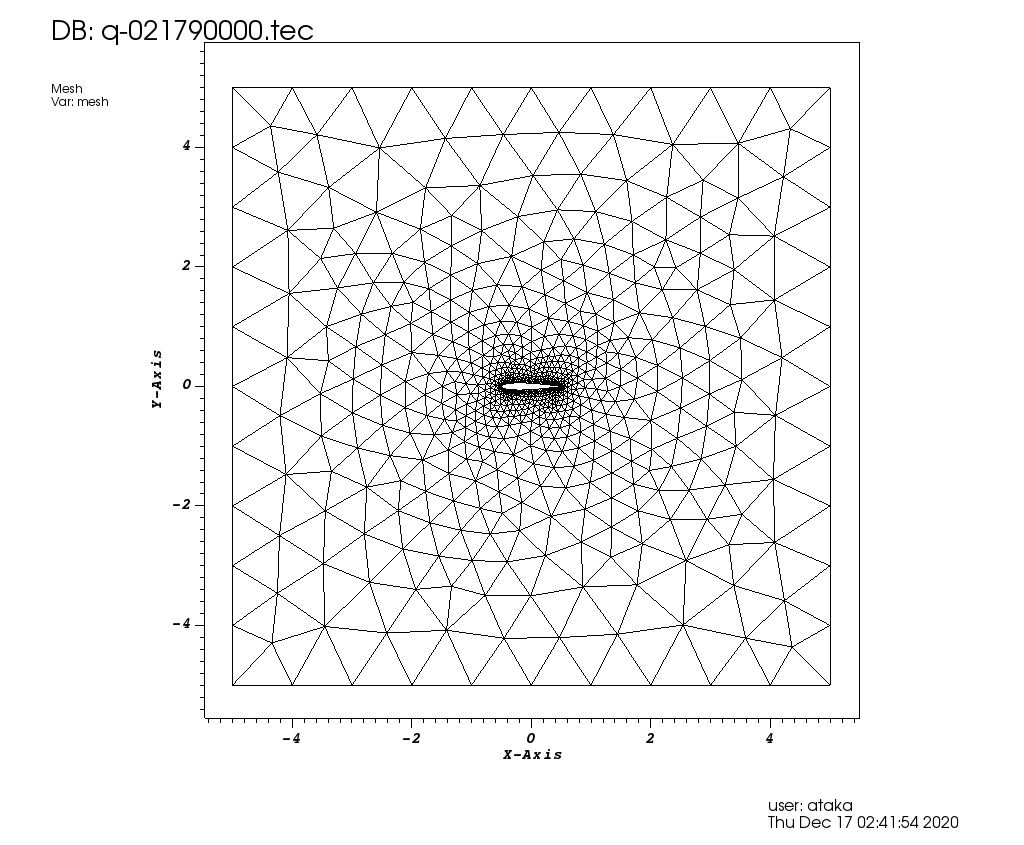
\includegraphics[height = 9.5cm]{graph/coarse/coarse_8470000.png}
	\caption{Coarse unstructured mesh of NACA0012 airfoil}
    \label{fig:airfoilmeshcoarse}
\end{figure}

\vspace{1cm}

Coarse unstructured mesh of NACA0012 airfoil is generated using Easymesh software. This
unstructured mesh consists of 847 triangular grids.

\newpage

\begin{figure} [!h]
	\centering
	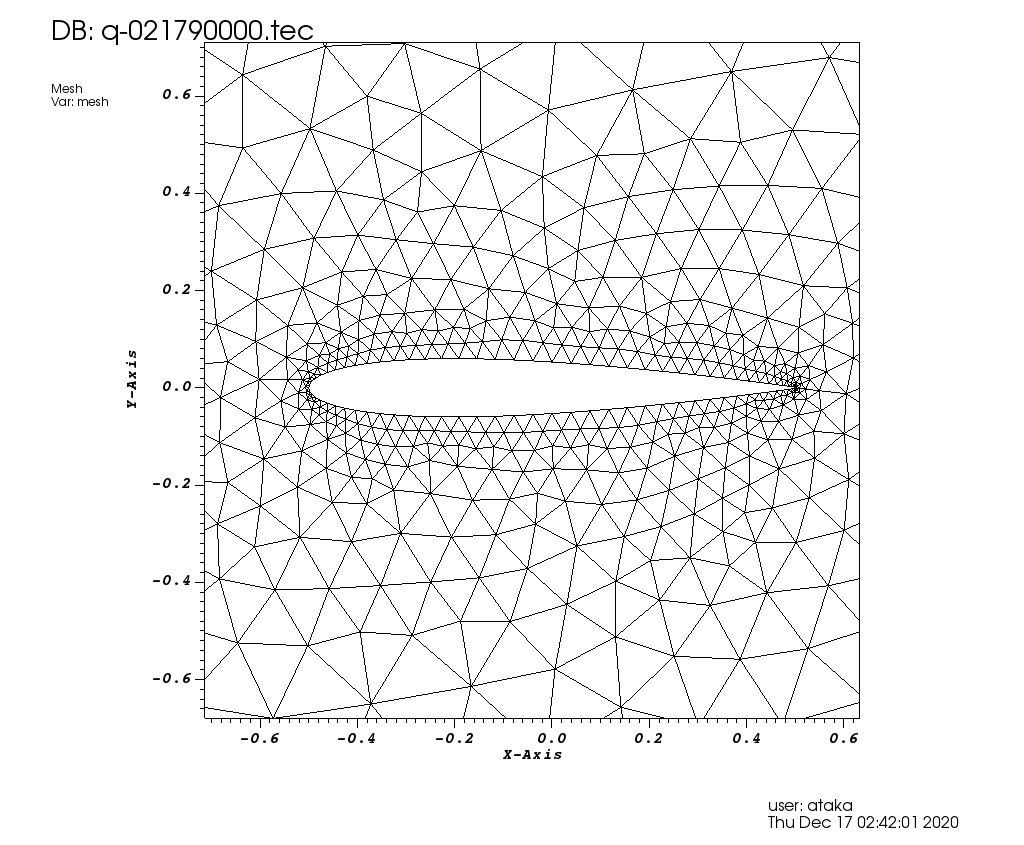
\includegraphics[height = 9.5cm]{graph/coarse/coarse_8470001.png}
	\caption{Coarse unstructured mesh of NACA0012 airfoil near the airfoil}
    \label{fig:airfoilmeshcoarseclose}
\end{figure}

\begin{figure} [!h]
	\centering
	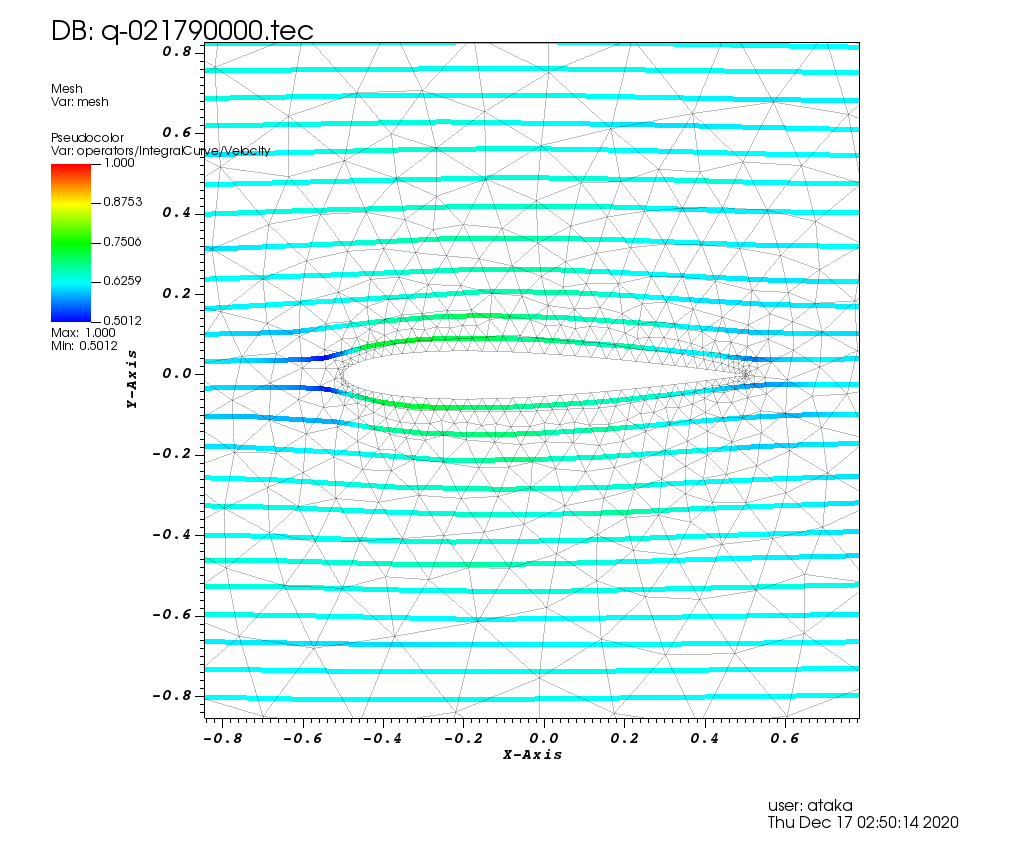
\includegraphics[height = 9.5cm]{graph/coarse/coarse_streamline0000.png}
	\caption{Streamlines around NACA0012 airfoil with coarse grid}
    \label{fig:airfoilcoarsestreamline}
\end{figure}

\newpage

It can be seen from Figure \ref{fig:airfoilcoarsestreamline} that, when coarse grid is 
used for calculation, streamlines obeys no penetration boundary condition but the magnitude 
of velocity is not calculated correctly around the airfoil.

\vspace{1cm}

\begin{figure} [!h]
	\centering
	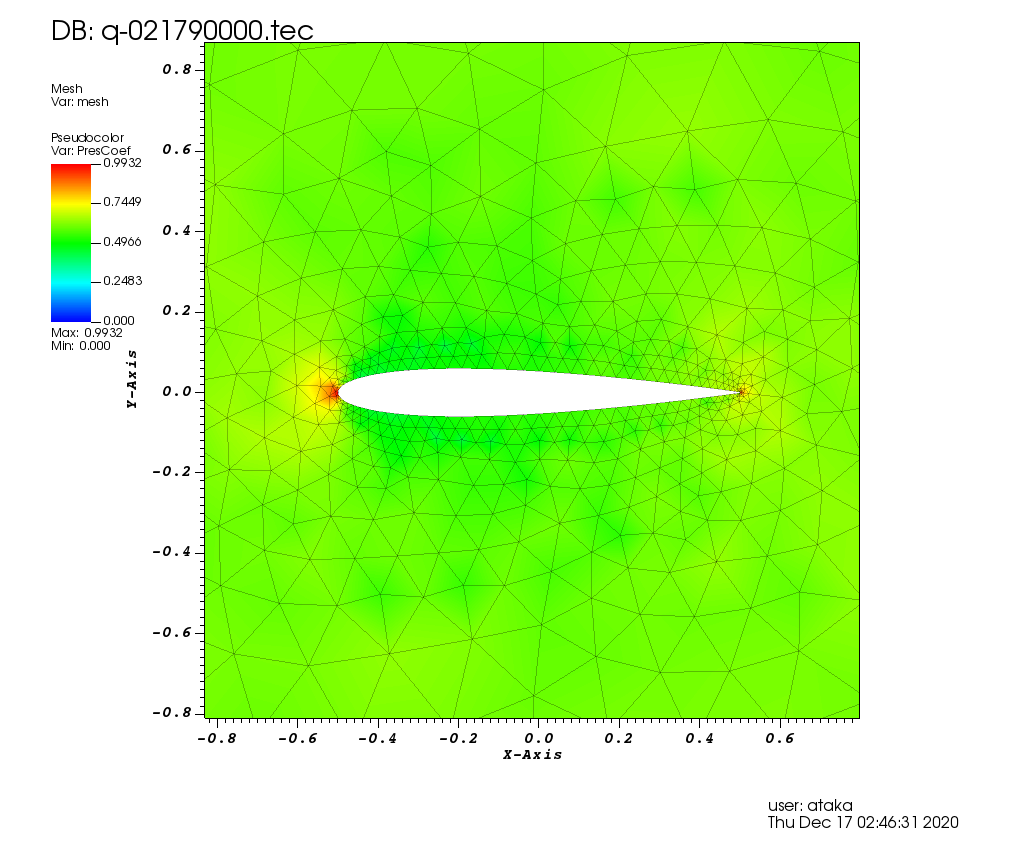
\includegraphics[height = 9.5cm]{graph/coarse/coarse_pressure0000.png}
	\caption{Pressure coefficient around NACA0012 airfoil with coarse grid}
    \label{fig:airfoilcoarsepressure}
\end{figure}

\vspace{1cm}

Around the leading and the trailing edge, pressure coefficient distribution is
closer to the correct distribution but still not correct enough. Around the maximum
thickness, the pressure distribution is way off the correct result. Therefore, the coarse
mesh is not suitable for a precise calculation of pressure around an airfoil.

\newpage

\subsubsection{Fine grid}

\begin{figure} [!h]
	\centering
	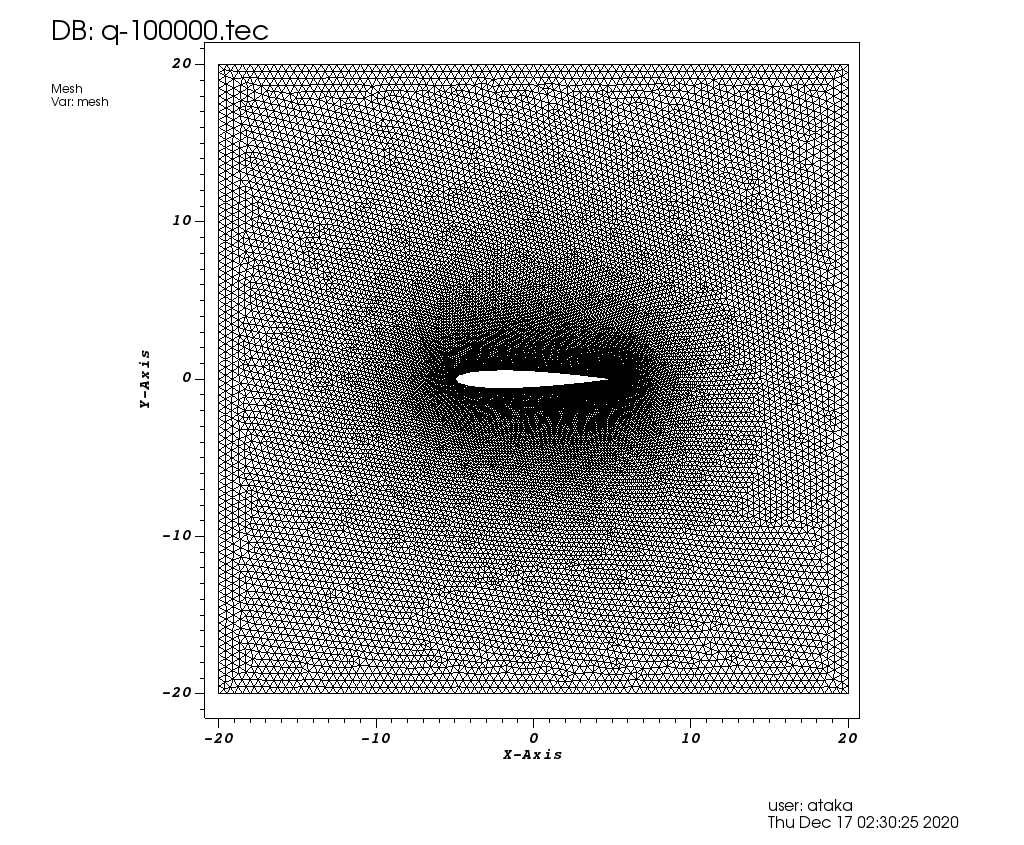
\includegraphics[height = 9.5cm]{graph/fine/fine_209480000.png}
	\caption{Fine unstructured mesh of NACA0012 airfoil}
    \label{fig:airfoilmeshfine}
\end{figure}

\vspace{1cm}

Fine unstructured mesh of NACA0012 airfoil is generated using Easymesh software. This 
unstructured mesh consists of 20948 triangular grids.

\newpage

\begin{figure} [!h]
	\centering
	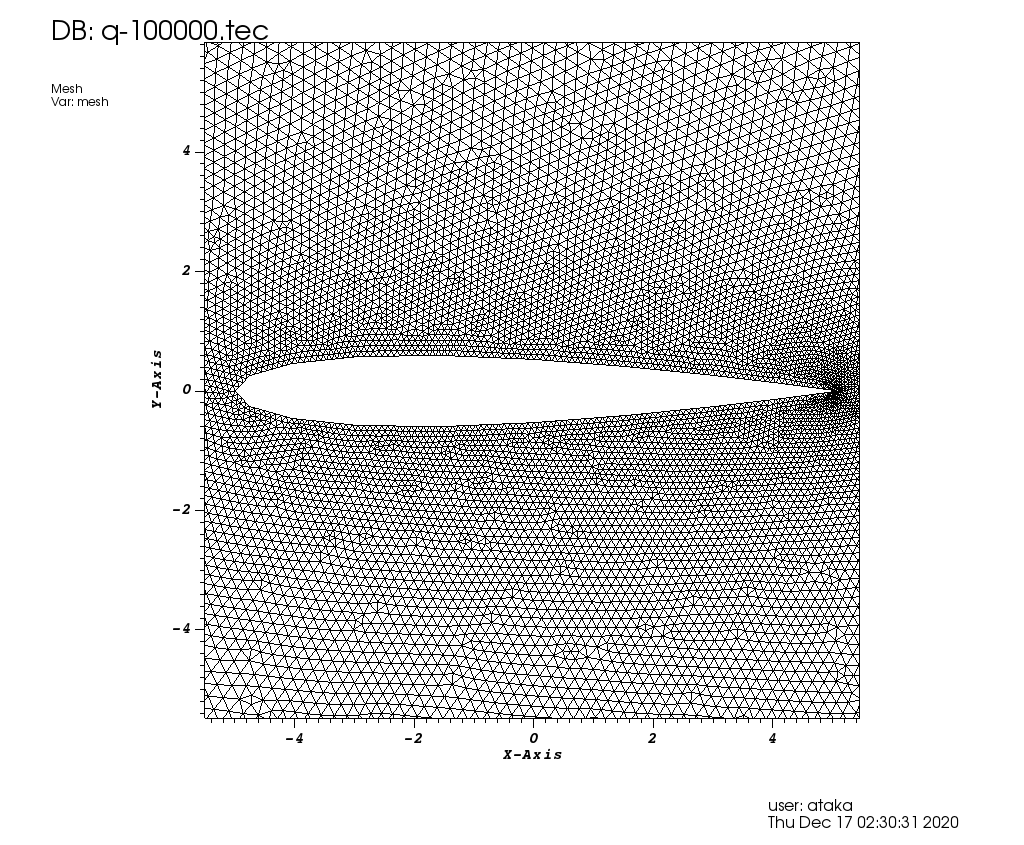
\includegraphics[height = 9.5cm]{graph/fine/fine_209480001.png}
	\caption{Fine unstructured mesh of NACA0012 airfoil near the airfoil}
    \label{fig:airfoilmeshfineclose}
\end{figure}
\begin{figure} [!h]
	\centering
	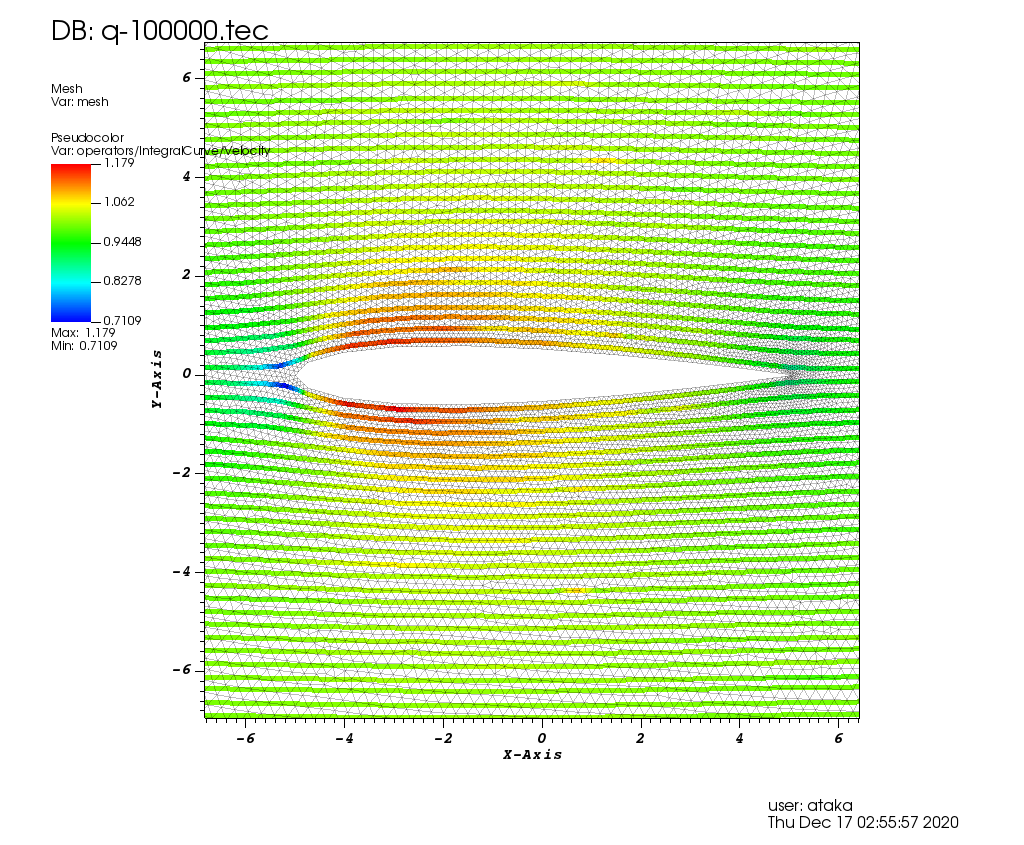
\includegraphics[height = 9.5cm]{graph/fine/fine_streamline0000.png}
	\caption{Streamlines around NACA0012 airfoil with fine grid}
    \label{fig:airfoilfinestreamline}
\end{figure}

\newpage

When a fine grid is used to calculate flow around the airfoil, the velocity distribution
can be found correctly around the airfoil. Figure \ref{fig:airfoilfinestreamline} 
illustrates that streamlines are calculated according to the no penetration boundary 
condition and air flows faster around the thicker part of the airfoil.

\vspace{1cm}

\begin{figure} [!h]
	\centering
	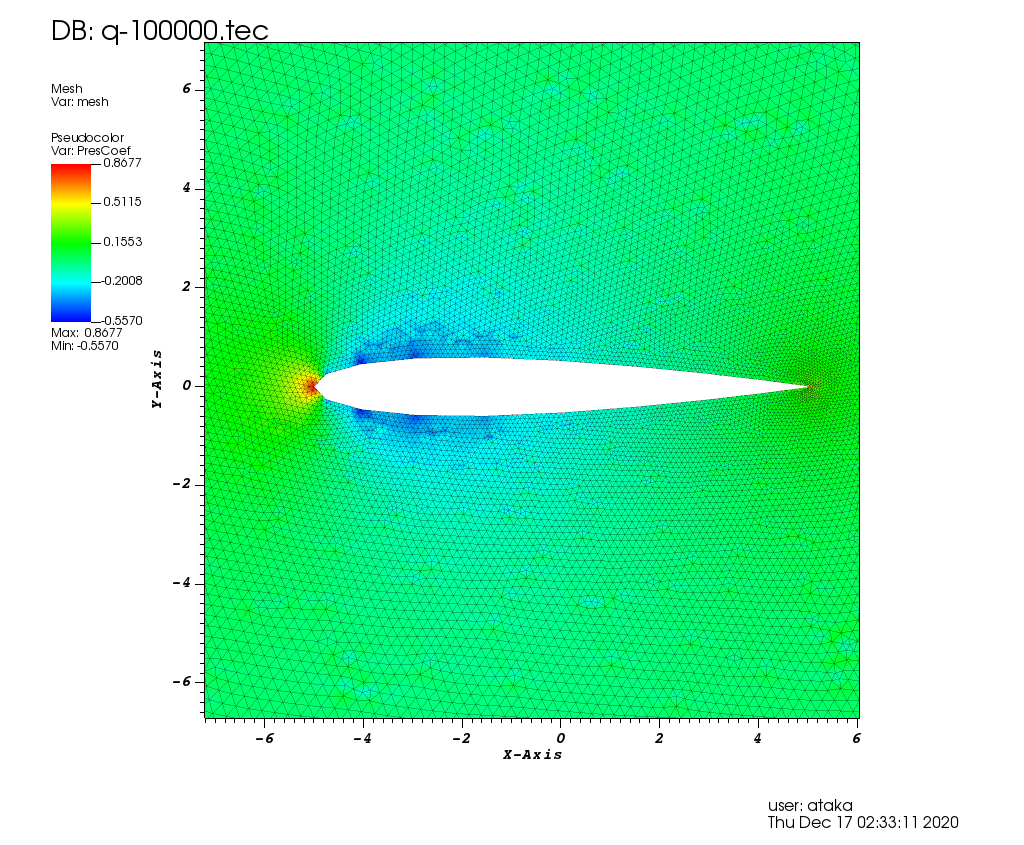
\includegraphics[height = 9.5cm]{graph/fine/fine_pressure0000.png}
	\caption{Pressure coefficient around NACA0012 airfoil with fine grid}
    \label{fig:airfoilfinepressure}
\end{figure}

\vspace{1cm}

As Figure \ref{fig:airfoilfinepressure} shows, the pressure distribution can be 
calculated more precisely when a finer grid is used. But the usage of finer grid
greatly increases the computation time, so unnecessarily fine grid should be avoided 
to maximize efficiency.

\subsubsection{Medium grid}

Calculations of Section \ref{sec:medium} is done using a medium grid, which consists of 
6255 triangular grids. When the results of this section are considered, it can be seen that
the medium grid is precise enough to give correct results and because of its relatively
lower triangle count, the result can be calculated faster. Therefore, using a medium grid
is more efficient.

\newpage

\section{Conclusion}

Given an unstructured grid of a circular cylinder, the potential flow, and the pressure 
coefficient distribution around it are requested to be calculated in the first part of
the problem. Afterwards, it is asked to replace the circular cylinder with a symmetric
NACA airfoil and repeat the calculations made for the cylinder in the second part of the
problem with coarse, medium, and fine grids.

First, the FV method fortran code is completed according to the steady-state boundary
conditions and compiled for the circular cylinder. It was observed that the flow velocity
is equal to the free stream velocity at farfield and its normal component to the surface
of the cylinder is zero, which implies that the boundary conditions are satisfied. Comparing
the pressure coefficient distribution obtained by the FV method with the analytical solution,
the points where the minimum and the maximum pressure occurs are the same for both solutions.

In the second part of the problem, an unstructured grid of the NACA0012 airfoil is obtained
using Easymesh software in order to replace the circular cylinder. The calculations were repeated,
and the potential flow and the pressure distribution are plotted also for the airfoil.
According to the observations made, the results for the airfoil were similar to that of
the cylinder. Boundary conditions were satisfied at farfield as well as at the boundary of
the airfoil. The plot of the pressure coefficient distribution calculated by Bernoulli's
equation illustrates that the $C_{p}$ values are the same for the upper and lower boundaries
resulting from the symmetry of the airfoil, and the minimum pressure coefficients occurred at
the leading and the trailing edges where the stagnations points are, as expected. 

Finally, the grid size used for the mesh is an important issue. Using coarse grids makes the calculation
faster but yields incorrect results. In contrast, fine grids enable to obtain accurate results
but the calculation duration is too long. Therefore, medium sized grids are used for the calculations
of this problem in order to approach the correct answer more precisely than the coarse grids could do,
and also in a relatively shorter time than the time needed for fine grids.
\end{document}